\chapter{Non-parametric dynamic system using AIS tracking data}
One of the significant issues with the direct approach is the unimodal assumption of using a \acrshort{gp}. It works well as long as vessels agree on a specific trajectory but fails as soon as there are multiple branching trajectories.

In \cite{pedestrian}, a \acrshort{gp} was used to model the trajectory patterns of pedestrians tracked using computer vision. Rather than directly describing trajectories, the paper proposed to simulate trajectories from a non-parametric dynamical model $\Delta\boldsymbol{x}_{t+1} = \vec{f}(\boldsymbol{x}_t)$ where the increments are expressed using a \acrshort{gp}. The trajectories were then simulated using two different approaches:
\begin{enumerate}
    \item By assuming $p(\boldsymbol{x})$ is always uni-modal and Gaussian, the GP-EKF introduced in \cite{gpekf} was used to simulate the trajectory for multiple timesteps, using the dynamical \acrshort{gp} model as the prediction model. This formulation is unable to express multimodal uncertainty.
    \item To retain the inherent multimodality, a sequential Monte-Carlo approach (i.e., the prediction step of a particle filter) was used to keep track of multiple modes (i.e., branching trajectories) at the cost of computational complexity.
\end{enumerate}

In this section, a similar method is proposed for long-term vessel prediction. The vessel trajectory $\boldsymbol{\mathcal{T}}$ can be expressed using the dynamical system
\begin{subequations}
    \begin{align}
        \boldsymbol{x}_{t+1} & = \boldsymbol{x}_t + \vec{f}(\boldsymbol{x}_t,t)                              \\
        \mathcal{T}_t        & = \boldsymbol{x}_t + \epsilon, \quad \epsilon \sim \mathcal{N}(0, \sigma^2)
    \end{align}
\end{subequations}
The function $\vec{f}(\cdot): \mathcal{R}^3 \to \mathcal{R}^2$ denotes the vector field describing the expected velocity. In the case of long-term prediction, the dynamics $\vec{f}(\cdot)$ is unknown and is unlikely to be stationary. Instead of using the usual parametric approaches to ODE models, the goal of this chapter is to use a \acrshort{gp} to create a non-parametric representation of the dynamics $\vec{f}(\cdot)$ by learning from historical trajectories of other vessels. This way, arbitrary complex dynamics can be learned without being limited by parametrization.

\begin{equation}\label{eq:gp_vec_field}
    \vec{f}(\boldsymbol{x}, t) = \vec{f}(\boldsymbol{\eta}) = \begin{bmatrix} f_x (\boldsymbol{\eta})\\ f_y (\boldsymbol{\eta})\end{bmatrix} \sim \text{GP} \big(\begin{bmatrix} m_x(\boldsymbol{\eta})\\m_y(\boldsymbol{\eta})\end{bmatrix}, \ \begin{bmatrix}
            K_{xx}(\boldsymbol{\eta}, \boldsymbol{\eta}') & K_{xy}(\boldsymbol{\eta}, \boldsymbol{\eta}') \\ K_{xy}(\boldsymbol{\eta}, \boldsymbol{\eta}')^\intercal & K_{yy}(\boldsymbol{\eta}, \boldsymbol{\eta}')
        \end{bmatrix}\big)
\end{equation}

The benefits of this formulation include:
\begin{description}
    \item[Easy incorporation of existing data] The model can easily be trained on partial data. Only the gradients of any historical trajectories are really needed.
    \item[Few constraining assumptions] The dynamical model is not constrained by any specific parametrization while still allows prior knowledge such as smoothness to be incorporated into the model.
    \item[Branching trajectories] The dynamical formulation only assumes Gaussian increments, while the full trajectory may still be multimodal. Though not analytically tractable, the multimodal trajectory can be found using sampling-based methods.
\end{description}

However, the major downside is that the model only learns gradients from data and relies heavily on numerical simulations to get the desired trajectories.

The model could further be improved by clustering the samples based on similar behavior for different ships, such as similar initial course and velocity. Separate \acrshort{gp}s could then be trained on the different subsets of data.

\section{Simulating trajectories using the Gaussian Process Extended Kalman Filter}

\subsection{EKF trajectory prediction}
Once the dynamics $\vec{f}_*$ is conditioned on data, it can be used to predict trajectories using the prediction procedure used by \textit{\acrfull{ekf}}. The combination of \acrshort{gp}s and \acrshort{ekf} was proposed by \cite{gpekf} and is summarized here. The reader is assumed to be already familiar with the Kalman filter and, by extension, the \acrshort{ekf}.

During the prediction procedure, the state is updated incrementally by adding $\vec{f}$ to the current state, i.e. the \acrshort{ekf} prediction model, $g(\boldsymbol{x})$, is given by \cref{eq:gp_ekf_prediction}.

\begin{equation}\label{eq:gp_ekf_prediction}
    \hat{\boldsymbol{x}}_{t} = \boldsymbol{g}_t(\boldsymbol{x}_{t-1}) = \boldsymbol{x}_{t-1} + \vec{f}(\boldsymbol{x}_{t-1}, t)
\end{equation}

Due to the potentially non-linear dynamics of $\vec{f}$, which implies non-linearity in $\boldsymbol{g}(\cdot)$, we need to linearize the prediction in order to propagate the state uncertianty $\boldsymbol{P}_{t-1}$. The Jacobian of the prediction model, $\boldsymbol{G}_t$, is given by \cref{eq:gp_ekf_prediction_jac} where the jacobian of $\vec{f}_*$ can be computed using \cref{eq:gp_jacobian}. We also define $\boldsymbol{\eta} \triangleq \begin{bmatrix}
    \boldsymbol{x} & t
\end{bmatrix}$ to simplify the notation for the \acrshort{gp} inputs. 

\begin{equation}\label{eq:gp_ekf_prediction_jac}
    \boldsymbol{G}_t = \frac{\partial \boldsymbol{g}_t(\boldsymbol{x}_{t-1})}{\partial \boldsymbol{x}_{t-1}} = I + \frac{\partial \vec{f}(\boldsymbol{x}_{t-1}, t)}{\partial \boldsymbol{x}_{t-1}}
\end{equation}

\begin{align}\label{eq:gp_jacobian}
    \begin{split}
        \frac{\partial \vec{f}(\boldsymbol{x}_*, t)}{\partial \boldsymbol{x}_*} &= \frac{\partial \vec{f}(\boldsymbol{\eta})}{\partial \boldsymbol{x}_*} \\  &= \frac{\partial}{\partial \boldsymbol{x}_*} \bigg(\boldsymbol{k}_*^\intercal K^{-1} \big(\boldsymbol{y} - m(X)\big)\bigg)\\
        &= \frac{\partial \boldsymbol{k}_*^\intercal}{\partial \boldsymbol{x}_*} K^{-1} \big(\boldsymbol{y} - m(X)\big)\\
        &= \frac{\partial \boldsymbol{k}_*^\intercal}{\partial \boldsymbol{x}_*} \boldsymbol{\alpha} = \begin{bmatrix}
            \frac{\partial k(\boldsymbol{\eta}_*, \boldsymbol{\eta}_1)}{\partial \boldsymbol{x}_*[1]} & \frac{\partial k(\boldsymbol{\eta}_*, \boldsymbol{\eta}_1)}{\partial \boldsymbol{x}_*[2]} \\
            \frac{\partial k(\boldsymbol{\eta}_*, \boldsymbol{\eta}_2)}{\partial \boldsymbol{x}_*[1]} & \frac{\partial k(\boldsymbol{\eta}_*, \boldsymbol{\eta}_2)}{\partial \boldsymbol{x}_*[2]} \\
            \vdots & \vdots \\
            \frac{\partial k(\boldsymbol{\eta}_*, \boldsymbol{\eta}_N)}{\partial \boldsymbol{x}_*[1]} & \frac{\partial k(\boldsymbol{\eta}_*, \boldsymbol{\eta}_N)}{\partial \boldsymbol{x}_*[2]} \\
        \end{bmatrix}^\intercal \boldsymbol{\alpha}
    \end{split}
\end{align}

We can then predict the state uncertainty using \cref{eq:gp_ekf_prediction_uncertianty}, propagating the previous uncertainty $\boldsymbol{P}_{t-1}$ using the linearized prediction model $\boldsymbol{G}_t$ and adding the prediction uncertianty $\mathbb{V}[\vec{f}]$.

\begin{equation}\label{eq:gp_ekf_prediction_uncertianty}
    \boldsymbol{P}_t = \boldsymbol{G}_t^\intercal \boldsymbol{P}_{t-1} \boldsymbol{G}_t + \mathbb{V}[\vec{f}(\boldsymbol{x}_{t-1}, t)]
\end{equation}

The prediction procedure is summarized in \cref{alg:gp_ekf_prediction} and can be used iteratively to simulate a complete trajectory, as demonstrated in \cref{fig:gp_ekf}.

\begin{algorithm}[h]
    \begin{algorithmic}[1]
        \Procedure{GP-EKF-PREDICT}{$\vec{f}$, $\boldsymbol{x}_{t-1}$, $\boldsymbol{P}_{t-1}$, $\Delta t$}
        \State $\hat{\boldsymbol{x}}_{t} = \boldsymbol{x}_{t-1} + \mathbb{E}\big[\vec{f}(\boldsymbol{x}_{t-1}, t)\big] \Delta t$
        \State $\boldsymbol{G_t} = I + \frac{\partial \vec{f}(\boldsymbol{x}_{t-1}, t)}{\partial \boldsymbol{x}_{t-1}} \Delta t$
        \State $\hat{\boldsymbol{P}}_t = \boldsymbol{G_t}^\intercal \boldsymbol{P}_{t-1} \boldsymbol{G_t} +\mathbb{V}[\vec{f}(\boldsymbol{x}_{t-1}, t)] (\Delta t)^2$
        \State \textbf{return} $\hat{\boldsymbol{x}}_t, \; \hat{\boldsymbol{P}}_t$
        \EndProcedure
    \end{algorithmic}
    \caption{GP-EKF Trajectory Prediction}
    \label{alg:gp_ekf_prediction}
\end{algorithm}

\begin{figure}
    \centering
    \begin{subfigure}{\textwidth}
    \centering
    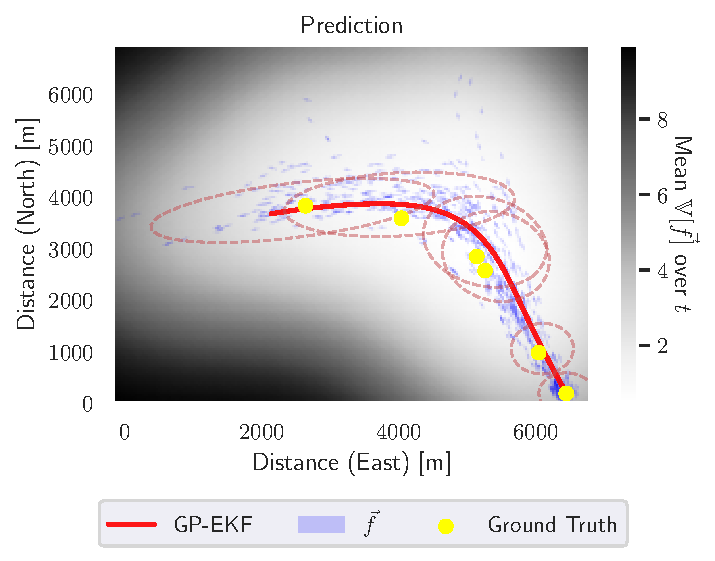
\includegraphics[width=\textwidth]{figures/dyngp/gp_ekf.pdf}
    \caption{Trajectory plotted against the vector-field $\vec{f}(\boldsymbol{x})$. The ellipses show the $95\%$ credibility interval for the predicted trajectory at the ground-truth timestamps.}
    \end{subfigure}
    \begin{subfigure}{\textwidth}
    \centering
    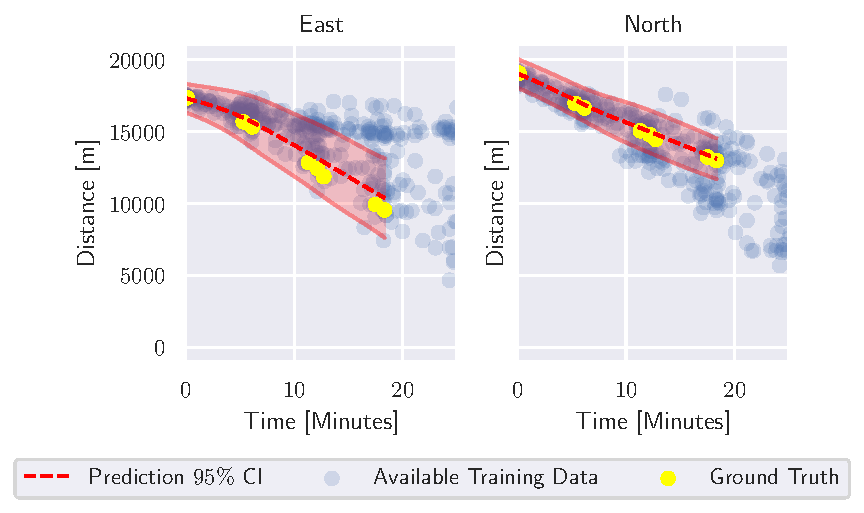
\includegraphics[width=\textwidth]{figures/dyngp/gp_ekf_state.pdf}
    \caption{$2\sigma$ credibility interval for the trajectory plotted against time}
    \end{subfigure}
    \caption{Predicted position using \cref{alg:gp_ekf_prediction}}
    \label{fig:gp_ekf}
\end{figure}


\subsection{Incorporating vessel position}
While the prediction procedure proposed in \cref{alg:gp_ekf_prediction} yields good predictions in many cases, it is inherently an open-loop prediction. Inaccurate predictions will never be corrected, propagating through any remaining iterations, potentially leading to significant errors later on. Looking at the available data in \cref{fig:gp_ekf_with_pdaf}, we want the prediction to converge towards available position measurements, \textit{slowly and only if the prediction is clearly wrong}. In other words, we want weak feedback that may compensate for minor prediction errors. 

As we do not have any actual position measurements of the vessel's future position, we need to express somehow that the available training data are \textbf{potential} measurements, which at any timestep may or may not originate from the vessel. Incorporating vessel position becomes a data association problem, for which we can look to target tracking for inspiration.

The \textit{\acrfull{pdaf}} is a method commonly used in target tracking which combines data association and filtering. The following introduction to \acrshort{pdaf} is mostly inspired by \cite{sensorfusjon}, with some adaptations to fit our problem better. As single target tracking and data association is not the topic of this thesis, only a short introduction to the \acrshort{pdaf} will be included here. For more details, see \cite{sensorfusjon,bar1995multitarget}

In this section, we will consider all measurements in the available training set as virtual \footnote{By virtual, we mean a measurement that did not actually originate from the target vessel, but rather a measurement that could potentially originate from our target in the future. The word measurement is still used to keep the terminology similar to what is used by \acrshort{pdaf}.} position measurements, which may or may not originate from the vessel at time $t$. We will use the same assumption as the \acrshort{pdaf}, where we assume \textbf{at most one} measurement originating from the target to reduce the computational complexity significantly \cite{sensorfusjon}. As we do not have proper measurements of the vessel's position in the future, we expect most of the measurements to be clutter, forcing the model to primarily trust its predictions. 

Given the predicted state $\hat{\boldsymbol{x}}_t$, we expect any real measurement to be distributed around this state due to some measurement noise. Following the notation used by \acrshort{ekf}, and using the measurement model $h(\boldsymbol{x}) = \boldsymbol{x} \implies H = \frac{\partial h (\boldsymbol{x})}{\partial \boldsymbol{x}} = I$, the predicted measurement distributed is expressed as in \cref{eq:gp_ekf_pdaf_measurement} where we define $\boldsymbol{S}_t \triangleq \hat{\boldsymbol{P}}_t + \boldsymbol{R}$ and $\boldsymbol{R}$ is the measurement noise.

\begin{equation} \label{eq:gp_ekf_pdaf_measurement}
    \hat{\boldsymbol{z}}_t \sim \mathcal{N}(\hat{\boldsymbol{x}}_t, \boldsymbol{S}_{t}) = \mathcal{N}(\hat{\boldsymbol{x}}_t, \hat{\boldsymbol{P}}_t + \boldsymbol{R})
\end{equation}

None of the measurements may originate from the target, i.e., we only observe clutter. The choice of a good clutter model is a complicated topic, but we will here use the Poisson clutter model. As the measurements are not actual measurements from our target, it is difficult to assign meaning to any clutter model. It, therefore, simply boils down to which parameters we need to tune\footnote{We here pretend that the trajectory prediction can be seen as a target tracking problem. The clutter parameters, therefore, need to be interpreted in the context of target tracking, not trajectory prediction.} and the Poisson clutter model should already be familiar to anyone with experience in target tracking.
According to the Poisson clutter model, the association probabilities are given by \cref{eq:pdaf_clutter_association_prob}, where $a_t$ is a discrete variable following a Categorical distribution where $a_t=k > 0$ denotes that measurement $k$ originated from the target. $a_t = 0$ is the special case when none of the measurements originated from the target, i.e., the predicted state should not be updated. $Z$ here denotes a matrix of all the measurements (positions) available in the training data and is independent of time, i.e., all measurements are always potential candidates. $\lambda$ denotes the clutter rate, and $P_D$ denotes the probability of detecting the target vessel.
\begin{equation}\label{eq:pdaf_clutter_association_prob}
    \Pr\{a_t | Z\} \propto \begin{cases}
        \lambda (1 - P_D) &  a_t = 0\\
        P_D \mathcal{N} (\boldsymbol{z}^{a_t} | \hat{\boldsymbol{x}}_t, \boldsymbol{S}_t) & a_t > 0\\
    \end{cases}
\end{equation}

Once we have the likelihood for each of the possible outcomes, the association probabilities $\boldsymbol{\beta}$ can be computed by normalizing the likelihood. 

\begin{equation}
    \beta_i = \frac{\Pr\{a_t=i \; | \; Z\}}{\sum_{k=0}^M \Pr\{a_t=k \; | \; Z\}}
\end{equation}

We can then update the predicted step using the Kalman update procedure, conditioned on the assocication $a_t$ and the updated state of the vessel can be described as a Gaussian Mixture Model over $M+1$ different modes weighted by the association probabilites, i.e. 
\begin{equation}
    p(\boldsymbol{x_t}) = \underbrace{\beta_0 \mathcal{N}(\boldsymbol{x}_t \; | \; \hat{\boldsymbol{x}}_t, \hat{\boldsymbol{P}}_t)}_{\text{No measurements are valid}} + \sum_{k=1}^M \underbrace{\beta_k \mathcal{N}\big(\boldsymbol{x}_t | \boldsymbol{x}_t^{a_k}, \boldsymbol{P}_t^{a_k}\big)}_{\text{Measurement $k$ is valid}}
\end{equation}

Moment reduction is then used to combined the different hypothesises into a single unimodal Gaussian distribution, i.e. we want to find a Gaussian distribution that matches the first and second moment (mean and variance) of the Gaussian mixture. The mean and variance of the resulting distribution is given by \cref{eq:pdaf_moment_mean} and \cref{eq:pdaf_moment_var} respectively, where we use $\boldsymbol{v}_t = \sum_{a_t > 0} \beta_t^{a_t} \boldsymbol{v}_t^{a_k}$. 

\begin{subequations}
\begin{align}
    \boldsymbol{x}_t &= \hat{\boldsymbol{x}}_t + \boldsymbol{W}_t \boldsymbol{v}_t \label{eq:pdaf_moment_mean}\\
    \begin{split}
    \boldsymbol{P}_t &= \hat{\boldsymbol{P}}_t - (1 - \beta_t^{0}) \boldsymbol{W}_t \boldsymbol{S}_t  \boldsymbol{W}_t\\ &+ \boldsymbol{W}_t \big[\sum_{a_t > 0}^M \beta_t^{a_t} \boldsymbol{v}_t^{a_t} (\boldsymbol{v}_t^{a_t})^\intercal - \boldsymbol{v}_t \boldsymbol{v}_t^\intercal \big] \boldsymbol{W}_t^\intercal\label{eq:pdaf_moment_var}
    \end{split}
\end{align}
\end{subequations}

While we could consider all available measurement at each timestep, it is in practice more convenient only to include a subset which is close enough to our predicted state. As we want this measurement \textit{gate} to scale with the uncertainty, we select the gated subset as \cref{eq:pdaf_gate} where $g$ is the number of standard deviations we want to consider.

\begin{equation} \label{eq:pdaf_gate}
    \mathcal{G} = \big\{ \boldsymbol{z} \; | \; (\boldsymbol{z} - \hat{\boldsymbol{x}}_t)^\intercal S^{-1} (\boldsymbol{z} - \hat{\boldsymbol{x}}_t) < g^2 \big\}
\end{equation}




Combining this update procedure with the GP-EKF prediction procedure in \cref{alg:gp_ekf_prediction}, the predicted trajectory can be tuned to favor areas with a large number of samples, effectively pulling the state towards areas with available samples. In regions with samples spread evenly around the predicted state, then the \acrshort{pdaf}'s effect is negligible (assuming proper tuning).

\begin{figure}
    \centering
    \begin{subfigure}{\textwidth}
    \centering
    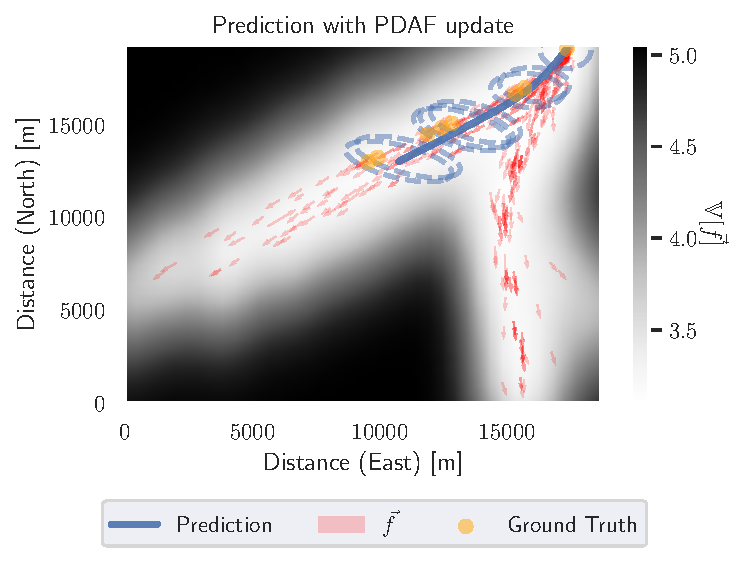
\includegraphics[width=\textwidth]{figures/dyngp/gp_ekf_with_pdaf.pdf}
    \caption{Trajectory plotted against the vector-field $\vec{f}(\boldsymbol{x})$. The ellipses show the $95\%$ credibility interval for the predicted trajectory at the ground-truth timestamps.}
    \end{subfigure}
    \begin{subfigure}{\textwidth}
    \centering
    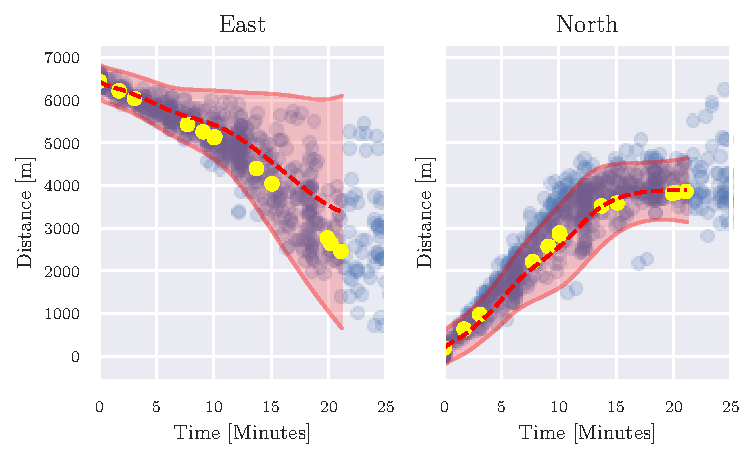
\includegraphics[width=\textwidth]{figures/dyngp/gp_ekf_with_pdaf_state.pdf}
    \caption{$95\%$ credibility interval for the trajectory plotted against time}
    \end{subfigure}
    \caption{Predicted position with the PDAF update procedure.}
    \label{fig:gp_ekf_with_pdaf}
\end{figure}

\subsubsection{Tuning PDAF parameters}
We want the model to prioritize the prediction model, as it would otherwise be stuck since the measurements do not change over time. As the measurements are not originating from the target vessel, we also expect a lot of noise in the measurements themselves. In practice, this boils down to using a significant measurement noise $\boldsymbol{R}$ and a relatively low detection probability $P_D$ before tuning the clutter rate to achieve good results. 
\subsubsection{Consistency}


\section{Simulating trajectories using Gaussian Process Sequential Monte Carlo}
The Kalman-based prediction scheme proposed in the previous section works well as long as a single Gaussian distribution can sufficiently explain the uncertainty. However, in branching trajectories, minor differences in position early in the predicted trajectory might have significant effects on the predicted state later on. The result is a multimodal trajectory distribution, which a Kalman-based approach is not able to express.

Inspired by the prediction step used by \textit{particle filters} \cite{sensorfusjon}, the idea of sampling trajectories can be used to explore the multimodal trajectory distribution. While inspired by the particle filter, this approach will from now on be referred to as \textit{Sequential Monte-Carlo} to avoid confusion\footnote{An important part of the particle filter is weighting the particles based on available measurements. As we only perform sampling of trajectories, Sequential Monte-Carlo seems like a better fit.}. and to follow the same naming convention as used by \cite{pedestrian}.

The derivation of the Sequential Monte-Carlo approach is embarrassingly simple as this method trades high computational complexity for more straightforward mathematics. Instead of analytical propagation of uncertainty, many trajectories are simulated through random sampling and used to express the uncertainty empirically. We can this way describe the uncertainty for any trajectory distribution, though at the cost of considerable computational complexity. We also lose the convenience of parametric distributions described using only a few parameters.

Given a set $N$ particles at time $t$, $\{\boldsymbol{x}^1_t, \boldsymbol{x}^2_t, \cdots, \boldsymbol{x}^N_t\}$, the next state can be sampled 

\begin{figure}
    \centering
    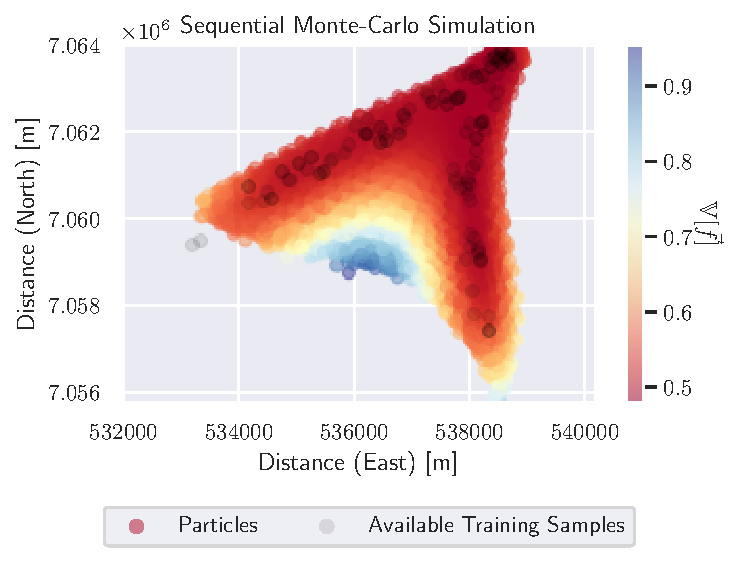
\includegraphics[width=\textwidth]{figures/dyngp/gp_particle.pdf}
    \caption{}
    \label{fig:gp_particle}
\end{figure}



